

%%%%%%%%%%%%%%%%%%%%%%%%%%%%%%%%%%%55%%
\begin{frame} [plain]
    \frametitle{}
    \Background[1] 
    \begin{center}
    {\huge 第8讲:量子通信 }
    \end{center}  
    \addtocounter{framenumber}{-1}   
\end{frame}
%%%%%%%%%%%%%%%%%%%%%%%%%%%%%%%%%%

\section{1.量子通信基础}
\begin{frame}
    \frametitle{量子通信网络}
    \begin{center}
        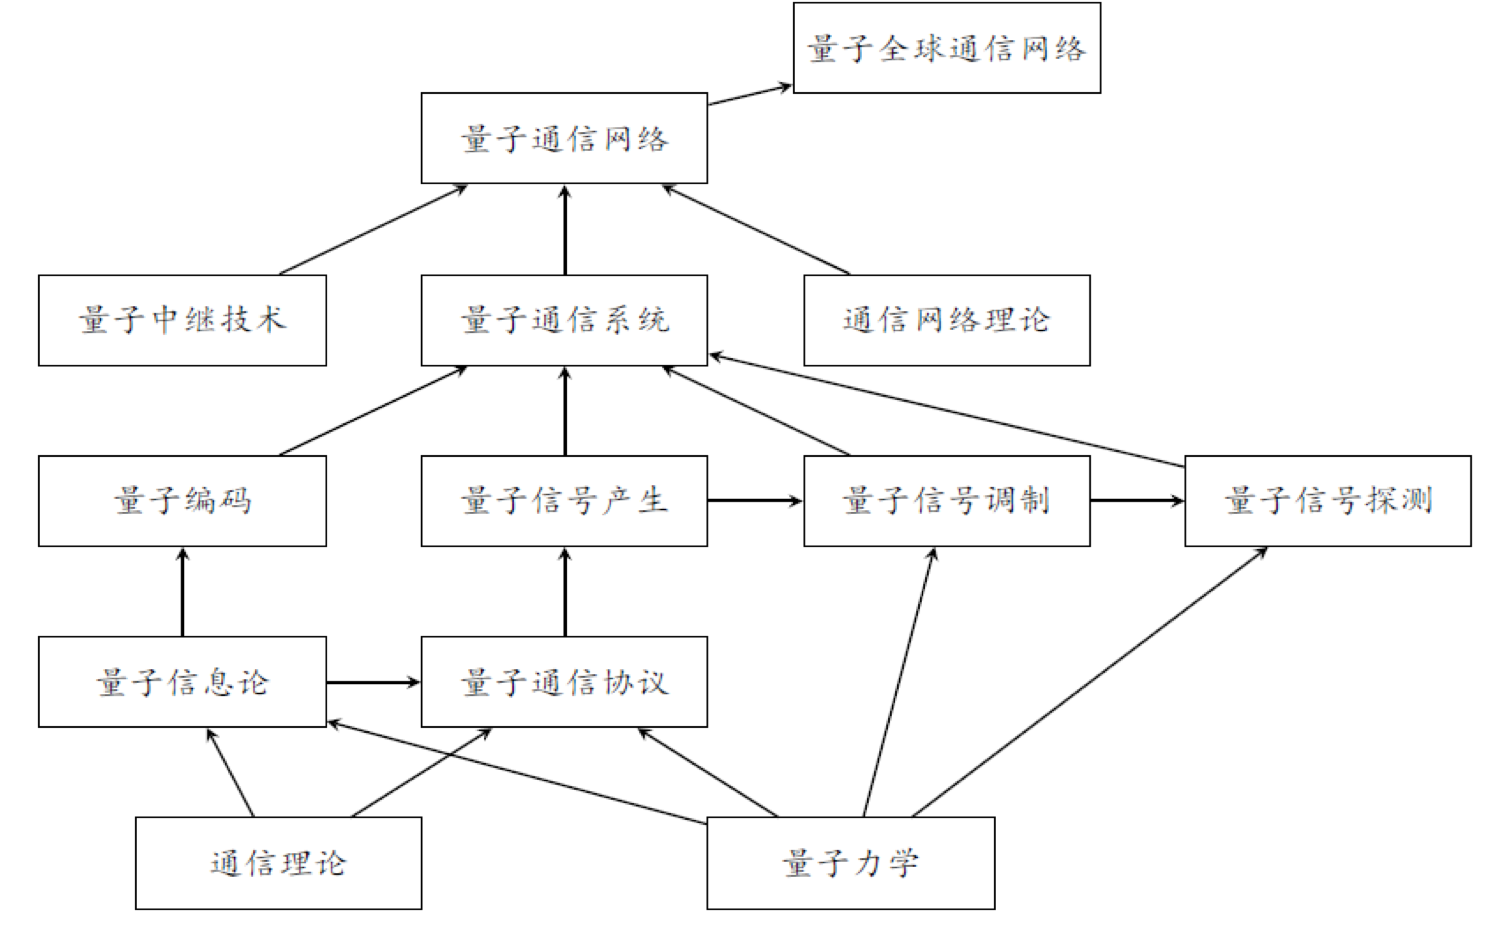
\includegraphics[width=0.85\textwidth]{figs/40.png}
    \end{center}
\end{frame}

\begin{frame}
    \frametitle{经典香农熵}
    假设一个事件有N种可能的结果,对应的概率分布为$\{p_k\}$,则香农熵定义为:
    \[H(x)=\sum_{k=1}^{N} p_{k} \log _{2} \frac{1}{p_{k}} \text { (bit) }\]
    代表测得可获取信息量的平均值\\
    对于2态事件,有:
    \[\begin{aligned} H_{2} &=p_{0} \log _{2} \frac{1}{p_{0}}+p_{1} \log _{2} \frac{1}{p_{1}} \\ 
        &=p \log _{2} \frac{1}{p}+(1-p) \log _{2} \frac{1}{(1-p)} \\
        &=1; \quad \text{if} \quad p=\frac{1}{2}
     \end{aligned}\]   
\end{frame}

\begin{frame}
    \frametitle{量子Von Neumann熵}
    设体系第n个本征态出现的概率为$p_n$,则密度矩阵和熵分别定义为:
    \[\rho=\sum_{n=1} p_{n}|n\rangle\langle n| \]
    \[S(\rho)=-\operatorname{tr}\left(\rho \log _{2} \rho\right)\]
    对于双粒子体系:有
    \[S\left(\rho_{A B}\right)=-\operatorname{tr}\left(\rho_{A B} \log _{2} \rho_{A B}\right)\]
    \[S\left(\rho_{A} \otimes \rho_{B}\right)=S\left(\rho_{A}\right)+S\left(\rho_{B}\right)\]
    \[S\left(\rho_{A} ; \rho_{B}\right)=\left[S\left(\rho_{A}\right)+S\left(\rho_{B}\right)\right]-S\left(\rho_{A B}\right)\]
\end{frame}

\begin{frame}
    \frametitle{密钥密码体系}
    \begin{itemize}
        \item  原文: I love you
        \item  密文: M PSZI CSY
        \item  加码函数: $f(x)=x+\alpha \bmod 26$
        \item  解码函数: $f^{-1}(y)=y-\alpha \bmod 26$
        \Item  密钥:$\alpha=4$ \\
        \item  原文序列:abcd{\color{red}{e}}fgh{\color{red}{i}}jk{\color{red}{l}}mn{\color{red}{o}}pqrst{\color{red}{u}}{\color{red}{v}}wx{\color{red}{y}}z \\
        \item  密文序列:ab{\color{green}{c}}defgh{\color{green}{i}}jkl{\color{green}{m}}no{\color{green}{p}}qr{\color{green}{s}}tuvwx{\color{green}{y}}{\color{green}{z}} \\ \vspace{1em}
        请问有多少个可能密钥?
    \end{itemize}
\end{frame}

\begin{frame}
    \frametitle{单时拍密钥方案}
    \begin{itemize}
        \item 原文字符串长度为$n$ \[ a_1a_2a_3\ldots a_n\]
        \item 信息发送者制备一个长度也为$n$的密钥串 \[ b_1b_2b_3\ldots b_n\]
        \item 加密函数 \[ c_i=a_i+b_i \bmod N \]
        \item 密文串 \[ c_1c_2c_3\ldots c_n\]
        \item 解密函数 \[ a_i=c_i-b_i \bmod N \]
    \end{itemize}
\end{frame}

\begin{frame}
    \frametitle{公开钥密方案}
    \begin{itemize}
        \item RSA密码方案: R.L.Rivest,A.Shamir和 L.Adelman于1978年提出的
        \item 依据:“验证两个大素数容易,而将他们的乘积做因数分解则极其困难” 
        \item 原文: $X$
        \item 密文: $Y$
        \item 加密: 使用公钥($e,N$) $Y=X^{e} \bmod N$
        \item 解密:使用私钥($d,N$) $X=Y^{d} \bmod N$
    \end{itemize}
\end{frame}

\begin{frame}
    \frametitle{}
    {\color{red}{制备}}:(e,d,N)
    \begin{enumerate}
        \item 秘密选择两个大素数$p,q$
        \item 计算出$N=p\times q$
        \item 计算出欧拉函数$\Phi(N)=(p-1)\times (q-1)$
        \item 选择一个较小的素数$e$做为公钥,它与$\Phi(N)$互质
        \item 计算私钥$d$, $ed\equiv 1 \mod \Phi(N)$
    \end{enumerate}
     {\color{red}{破解}}:想从$e$得到$d$,必须知道$\Phi(N)$;想要得到$\Phi(N)$,必须知道$p,q$; 想要得到$p,q$,必须做大数质因式分解$N=p \times q$!
\end{frame}


\begin{frame}
    \frametitle{密钥分发}
    \begin{itemize}
        \Item 密使分发 $\qquad$ 怕汉奸!
        \Item 公开分发 $\qquad$ 怕量子算法!
    \end{itemize}
    必须发展量子算法破解不了的量子密钥公开分发方案!
\end{frame}

\section{2.量子密码分发}
\subsection{量子不可克隆原理}
\begin{frame}
    \frametitle{量子不可克隆原理}
    {\Bullet}~克隆(cloning)指在目标系统(B)中产生一个与源系统(A)相同的态,而不改变源系统的态。\\ \vspace{1em}
    \例[1.试证明未知量子态不可克隆]{}
    \证~设已知的本征态可以克隆
    \[ U_c\rs{C}\rs{0}_A\rs{\varphi}_B=\rs{C_0}\rs{0}_A\rs{0}_B\]
    \[ U_c\rs{C}\rs{1}_A\rs{\varphi}_B=\rs{C_1}\rs{1}_A\rs{1}_B\]
    若A处于未知叠加态\[ \rs{\Psi}_A=\alpha\rs{0}+\beta\rs{1}\]
\end{frame}

\begin{frame}
    \frametitle{}
    期望的克隆:
    \[\begin{aligned}
        U_{c}|C\rangle|\psi\rangle_{A}|\varphi\rangle_{B}=&\left|C_{\psi}\right\rangle|\psi\rangle_{A}|\psi\rangle_{B} \\
        =&\left.\left|C_{\psi}\right\rangle(\alpha|0\rangle+\beta)|1\rangle\right)_{A}(\alpha|0\rangle+\beta|1\rangle)_{B} \\
        =&\left|C_{\psi}\right\rangle\left(\alpha^{2}|0\rangle_{A}|0\rangle_{B}+\alpha \beta|0\rangle_{A}|1\rangle_{B}+\alpha \beta|1\rangle_{A}|0\rangle_{B}\right.\\
        &~~\left.+\beta^{2}|1\rangle_{A}|1\rangle_{B}\right)
        \end{aligned} 
    \]
     服从量子力学的过程:
    \[ \begin{aligned}
        U_{c}|C\rangle|\psi\rangle_{A}|\varphi\rangle_{B} &=U_{c}|C\rangle\left(\alpha|0\rangle+\beta|1\rangle\right)_{A}|\varphi\rangle_{B} \\
        &=U_{c}|C\rangle \alpha|0\rangle_{A}|\varphi\rangle_{B}+U_{c}|C\rangle \beta|1\rangle_{A}|\varphi\rangle_{B} \\
        &=\alpha^{2}\left|C_{0}\right\rangle|0\rangle_{A}|0\rangle_{B}+\beta^{2}\left|C_{1}\right\rangle|1\rangle_{A}|1\rangle_{B}
        \end{aligned}
    \]
    ~~\\
    两式相等的必要条件为 $\alpha\beta=0$, 即可克隆的$\rs{\Psi}_A$态不可能是叠加态!\\
    证毕!          
\end{frame}

\subsection{量子不可删除原理}
\begin{frame}
    \frametitle{量子不可删除原理}
    {\Bullet}~删除是指如果目标系统(B)有源系统(A)的量子态副本,把B”置零” 而不改变A系统的状态
    \例[2.试证明未知量子态不可删除]{}
    \证~设已知的本征态可以删除
    \[ U_c\rs{C}\rs{0}_A\rs{0}_B=\rs{C_{00}}\rs{0}_A\rs{R}_B\]
    \[ U_c\rs{C}\rs{1}_A\rs{1}_B=\rs{C_{11}}\rs{1}_A\rs{R}_B\]
    \[ U_c\rs{C}\rs{0}_A\rs{1}_B=\rs{C_{01}}\rs{0}_A\rs{1}_B\]
    \[ U_c\rs{C}\rs{1}_A\rs{0}_B=\rs{C_{10}}\rs{1}_A\rs{0}_B\]
\end{frame}


\begin{frame}
    \frametitle{}
    对于叠加态,期望的删除:
    \[\begin{aligned}
        U_{c}|C\rangle|\psi\rangle_{A}|\psi\rangle_{B}&=\left|C_{\psi}\right\rangle|\psi\rangle_{A}|R\rangle_{B} \\
        &=|C_{\psi}\rangle(\alpha\rs{0}+\beta\rs{1})_{A}|R\rangle_{B} 
        \end{aligned} 
    \]
     服从量子力学的过程:
    \[ \begin{aligned}
        U_{c}|C\rangle|\psi\rangle_{A}|\psi\rangle_{B}=&U_{c}|C\rangle(\alpha|0\rangle+\beta|1\rangle)_{A}(|\alpha| 0\rangle+\beta|1\rangle)_{B} \\
        =& U_{c}|C\rangle \alpha^{2}|0\rangle_{A}|0\rangle_{B}+U_{c}|C\rangle \beta^{2}|1\rangle_{A}|1\rangle_{B} \\
        &~~+U_{c}|C\rangle \alpha \beta|0\rangle_{A}|1\rangle_{B}+U_{c}|C\rangle \alpha \beta|1\rangle_{A}|0\rangle_{B} \\
        =& \alpha^{2}\left|C_{00}\right\rangle|0\rangle_{A}|R\rangle_{B}+\beta^{2}\left|C_{11}\right\rangle|1\rangle_{A}|R\rangle_{B} \\
        &~~+\left|C_{01}\right\rangle \alpha \beta|0\rangle_{A}|1\rangle_{B}+\left|C_{10}\right\rangle \alpha \beta|1\rangle_{A}|0\rangle_{B}
        \end{aligned}
    \]
    ~~\\
    两式根本无法相等,即可删除的$\rs{\Psi}_A$态不可能是叠加态!\\
    证毕!          
\end{frame}

\subsection{BB84协议}
\begin{frame}
    \frametitle{}
    \begin{tcolorbox2}{BB84协议}
    {1984年,C. H. Bennett 和G. Brassard 提出利用偏振光进行量子密钥分发的协议。把一次性密码原理和量子测量原理结合在一起,建立不可破解密码分发方案}
    \end{tcolorbox2}  
\end{frame}

\begin{frame}
    \frametitle{原理}
    \begin{enumerate}
        \item Ailce 由随机数序列a决定选择纵横基还是对角基。设a中的0代表纵横基{$\rs{0},\rs{1}$},1代表对角基{$\rs{+},\rs{-}$} 
        \item Ailce 再由随机数序列a' 决定发射给Bob的光子的具体偏振。设a'中的0代表$\rs{0},\rs{+}$, 设a'中的1代表$\rs{1},\rs{-}$\\
        \hspace{2em} 设有 $a=0010$,$a'=1001$:Ailce发出的光子的偏振序列为$\rs{10+1}$
        \item Bob 得到偏振光子串后,由随机数序列b决定选择纵横基还是对角基,再由随机数序列b' 决定用相应基里的那个基矢波片进行测量\\
        \hspace{2em} 设有 $b=0110$,$b'=1100$:Bob使用的偏振片序列为$\rs{1-+0}$ 
        \item 双方公布第一序列(a=0010 and b=0110),发现第1、3位相同。
        \item 双方就知道各自手里的$a'=1001$和$b'=1100$中的第1、3位相同。整理出来,为$10$,并以此做为私钥d,完成密钥分发。
    \end{enumerate}
\end{frame}

\begin{frame}
  \frametitle{}
  \begin{figure}[htbp]
      \centering
      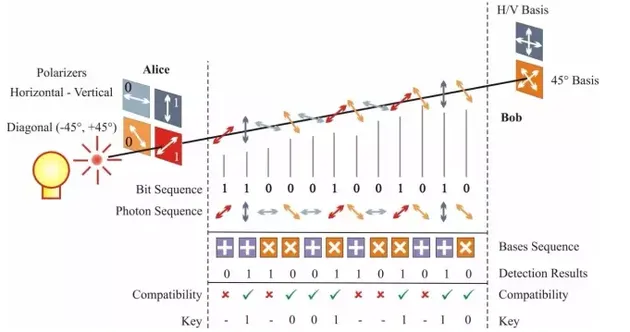
\includegraphics[width=0.9\textwidth]{figs/2022-03-17-00-33-08.png}
     % \caption{}
     % \label{}
  \end{figure}
\end{frame}


\begin{frame}
    \frametitle{}
    {\color{red}{保密性分析}}:
    \begin{enumerate}
        \item 设有窃听者C,先得到A发给B的每一个光子。这阻断了A、B之间的通信,没有得到d。
        \item C想知道光子的状态,若测量,因不知道具体的基,导致每个光子有$50\%$概率状态改变。
        \item C因不知光子状态,不能进行克隆,强行克隆势必导致原光子状态改变。
        \item C只能窃听Ailce和Bob的通信,得到a和b,但不是a'和b'。
        \item 派内鬼分别去Ailce和Bob的办公室,窃取a'和b',难度大于窃取d。
    \end{enumerate}
    (目前已走向实用!)
\end{frame}

\begin{frame}
  \frametitle{密钥增强技术}
  {\Bullet} 信息协调(Information Reconciliation):\\
  信息协调即密钥纠错(Error Correction),目的是保证Alice和Bob共同拥有的密钥的一致性。\\
  由于可能被C窃听,得保证公布的信息越少越好。而信道噪声或第三方窃听而导致的无效的部分进行删除,\\
  因此,信息协调后的密钥将更短。\\ \vspace{1em}
  {\Bullet} 隐私增强(Privacy Amplification):\\
  使密钥得以增强的一种方式,。\\
  (1) 公布的信息被窃听,(2) 信息协调被窃听, 窃听都知道的东西较多,有被破解的风险.比如排列组合!\\
  隐私增强即利用Alice和Bob手中的现有密钥,再生成一个新的、更短的密钥,相当于二次加密,增强破解难度.
\end{frame}

\begin{frame}
  \frametitle{}
\begin{figure}[htbp]
    \centering
    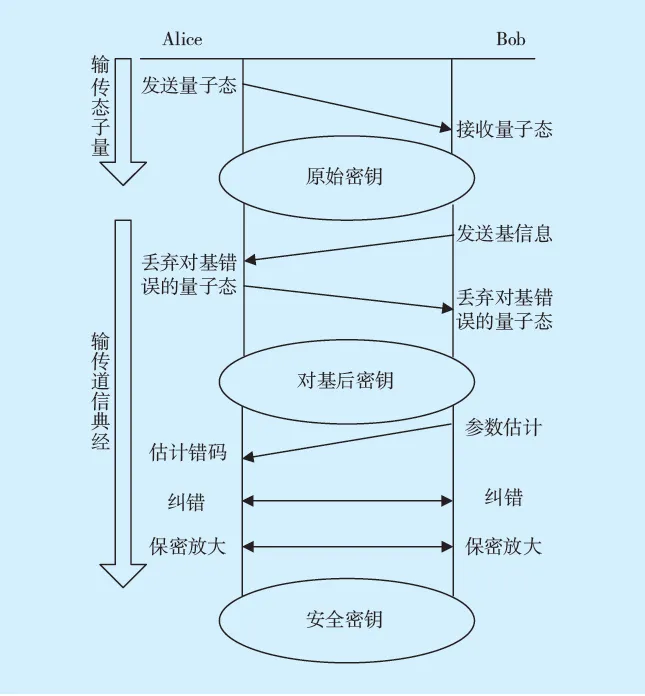
\includegraphics[width=0.6\textwidth]{figs/2022-03-17-00-41-14.png}
   % \caption{}
   % \label{}
\end{figure}
\end{frame}


\subsection{B92协议}
\begin{frame}
  \frametitle{B92协议}
  BB84协议要用四个偏振, 1992年,C.  H. Bennett 提出用两个非正交偏振态也可进行密码分发!\\ \vspace{0.6em}
  {\color{red}{原理:}} \\ \vspace{1em}
  (1) A 制备有二个偏振态
  \[ \rs{0}, \rs{-} \quad \to 0,1\]
因此有:
\[ \lr{-}{0}=\frac{\lr{0}{0}-\lr{1}{0}}{\sqrt{2}} =\frac{1}{\sqrt{2}} \]
\end{frame}

\begin{frame}
  \frametitle{}
 (2) B 有两个检测器
 \[ P_{-}=1-\rl{-}{-}\]
 \[ P_{0}=1-\rl{0}{0}\]
 (3) 若A发来的是$ \rs{0} $ 
    \[\lcr{0}{P_{-}}{0}=1\lr{0}{0}-\lr{0}{-}\lr{-}{0}=1-\frac{1}{2}=\frac{1}{2}\]
    若A发来的是$ \rs{-} $ 
    \[\lcr{-}{P_0}{-}=1\lr{-}{-}-\lr{-}{0}\lr{0}{-}=1-\frac{1}{2}=\frac{1}{2}\]
    即与BB84一样,0和1态的光子各以50\%的概率由A成功传送到B! 因此可用于密码分发.
\end{frame}

\begin{frame}
  \frametitle{专题研究:~E91协议}
  1991年, Eckert A.发布E91协议,它是基于EPR纠缠对实现密码分发的\\
   试分析其工作原理,并做出保密性分析
\end{frame}
